%Por Villa Fernández, Santiago; Gomez Vidal, Maximiliano, Sessa, Carlos, Abramowicz, Pablo

\documentclass[9pt]{beamer}

% \usetheme{Warsaw}
% \usecolortheme{default}
\usetheme{JuanLesPins}   % Beamer theme v 3.0
\usecolortheme{lily} % Beamer color theme

\usefonttheme{structurebold}
\useinnertheme{rounded}

\usepackage[spanish]{babel}
\usepackage[utf8]{inputenc}
\usepackage{amsmath}
\usepackage{amsfonts}
\usepackage{amssymb}
\usepackage{stmaryrd}
\usepackage{graphicx}

\usepackage{verbatim}

\setbeamercovered{transparent}

\title{Seguimiento de un blanco móvil}
\subtitle{Simulación de Sistemas}
\institute[ITBA]{
    ITBA \\
    Ciudad de Buenos Aires \\
}
\author{	Villa Fernández, Santiago  \and Gomez Vidal, Maximiliano  \\
				Sessa, Carlos  \and Abramowicz, Pablo}
\date{22 de Octubre de 2009}

\begin{document}

\frame{
    \titlepage
}

%================================== Outline ================================

\frame {
	\frametitle{Seguimiento de un blanco móvil}
	\tableofcontents[part=1]
}


\part{Seguimiento de un blanco móvil}

\section{Introducción}
	\subsection{Introducción}
		\frame{
			\frametitle{Introducción}
				\begin{center}
					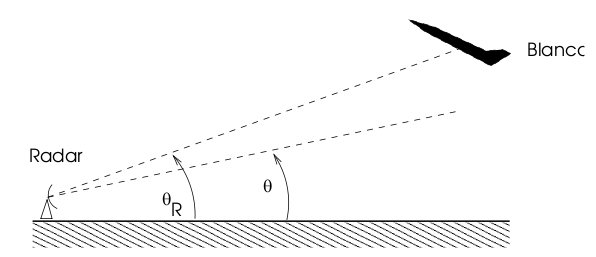
\includegraphics[scale=0.50]{./intro1.png}
				\end{center}
				\begin{block} {Resumen}
					Modelado de un sistema de seguimiento de blancos a lazo cerrado
					usando controladores de tipo proporcional, integral y derivativo.
				\end{block}

				\begin{block} {Objetivos}
					Determinar cuál es el controlador más eficiente.
				\end{block}
		}

\section{Modelado}

        \subsection{Dinámica de la antena}
			\frame{
				\frametitle{Dinámica de la antena}

				\begin{center}
					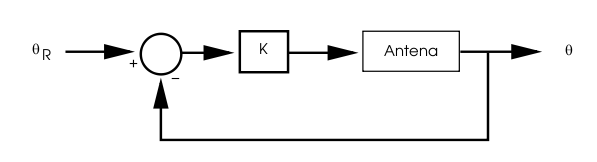
\includegraphics[scale=0.30]{./intro2.png}
				\end{center}

					\begin{block} {Dinámica de la antena}
						\begin{center}
							$I \ddot\theta = - b \dot\theta + u(t)$
						\end{center}

						\begin{itemize}
							\item $I = 0.004\ kg\ m^{2}$
							\item $b = 0.02\ kg\  m^{2}\ s^{-1}$
							\item $u(t)$ es el torque que producen los motores sobre la antena.
							\item El blanco se mueve según $\theta_{R}(t) = 0.01 t$
						\end{itemize}
					\end{block}

					\begin{block} {Error}
						\begin{center}
							$e(t) = \theta_{R}(t) - \theta(t)$
						\end{center}
					\end{block}
			}

\section{Controlador proporcional}
	\subsection{Modelo}
		\frame{
			\frametitle{\begin{center} $u(t) = K e(t)$ \end{center}}
			\begin{center}
% 				\framezoom<1><2>[border](-2.70cm,0cm)(1.5cm,1cm)
				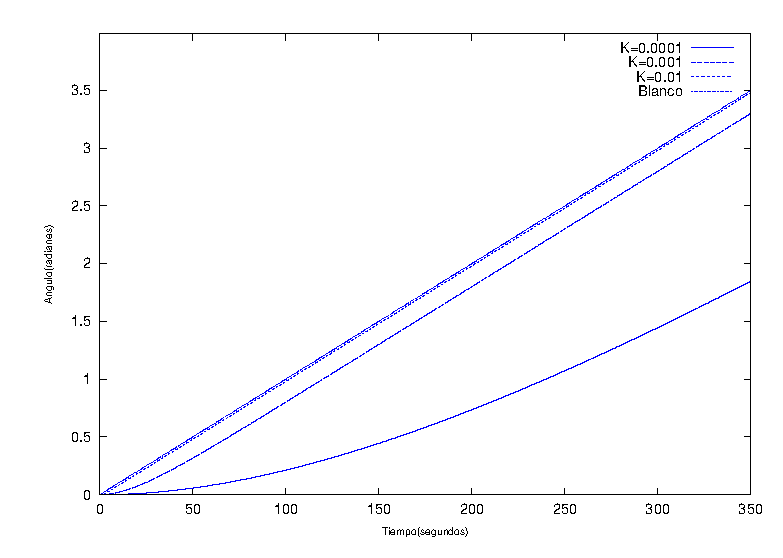
\includegraphics[height=6cm]{../graficos/mProporcional}
			\end{center}
		}

	\subsection{Error relativo porcentual}
		\frame{
			\begin{center}
				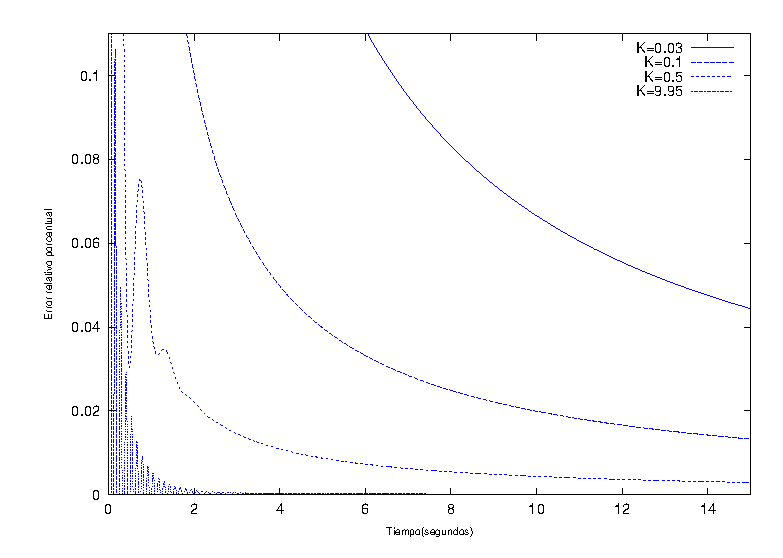
\includegraphics[scale=0.65]{../graficos/errorPorcentualMProporcional}
			\end{center}
		}

\section{Controlador integral}
	\subsection{Modelo}
		\frame{
			\frametitle{\begin{center} $u(t) = K_i \int_0^t e(\tau) d\tau$ \end{center}}
			\begin{center}
				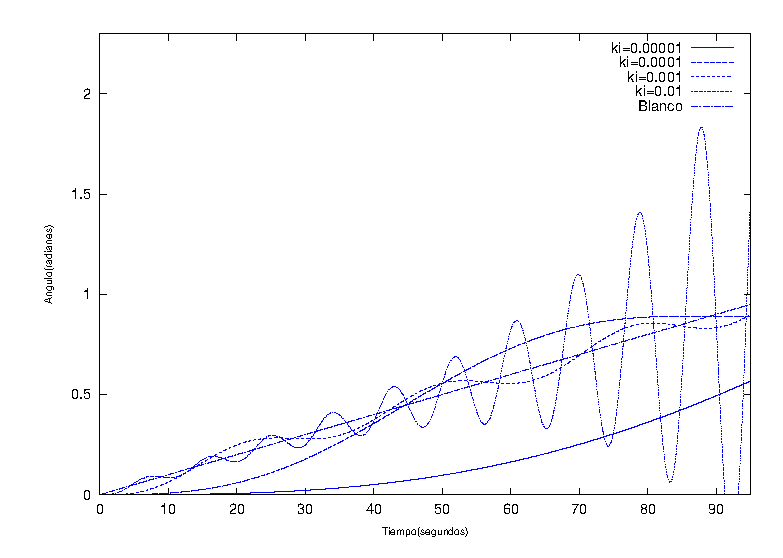
\includegraphics[scale=0.65]{../graficos/mIntegral}
			\end{center}
		}

	\subsection{Error relativo porcentual}
		\frame{
			\begin{center}
				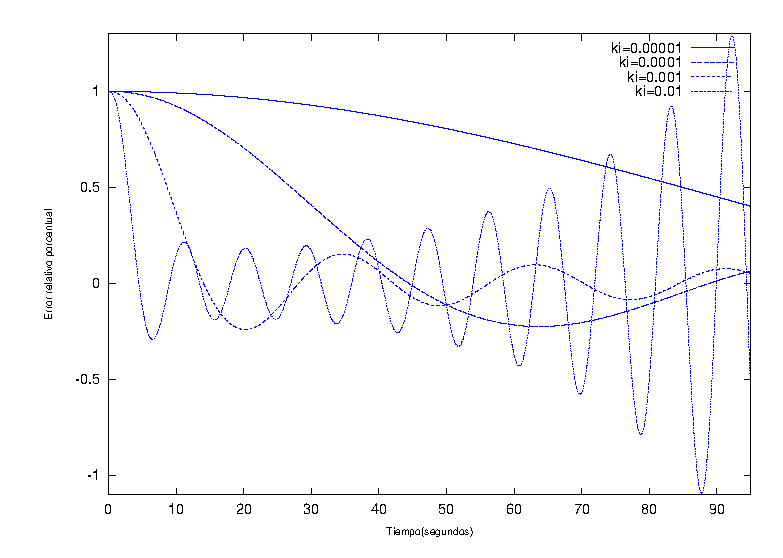
\includegraphics[scale=0.65]{../graficos/errorMIntegral}
			\end{center}
		}

\section{Controlador derivativo}
	\subsection{Modelo}
		\frame{
			\frametitle{\begin{center} $u(t) = K_d \frac{d e(t)}{d t}$ \end{center}}
			\begin{center}
				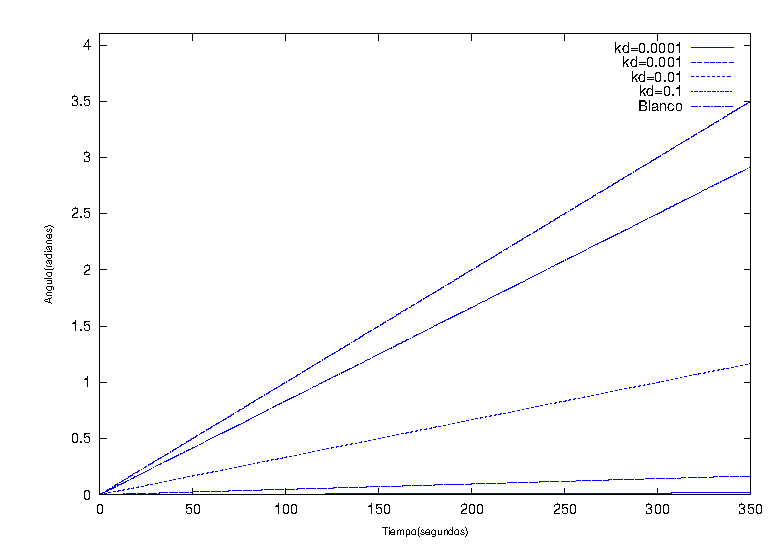
\includegraphics[scale=0.65]{../graficos/mDerivativo}
			\end{center}
		}

	\subsection{Error relativo porcentual}
		\frame{
			\begin{center}
				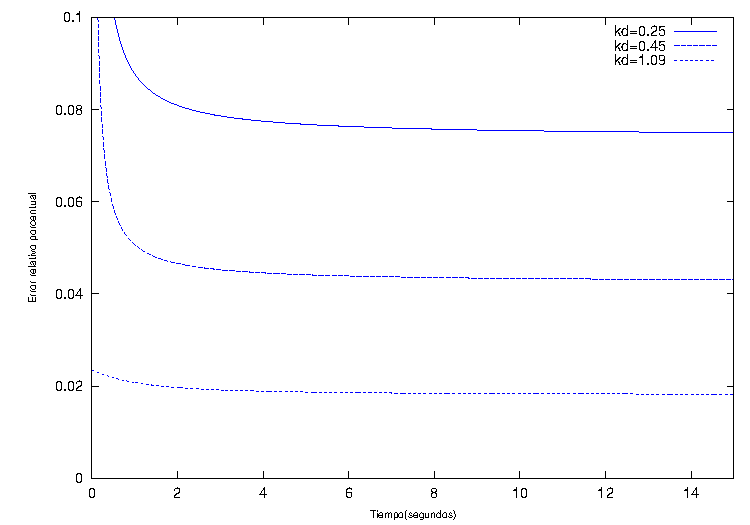
\includegraphics[scale=0.65]{../graficos/errorPorcentualMDerivativo}
			\end{center}
		}

\section{Conclusión}
	\subsection{Conclusión}
		\frame{
			\frametitle{Conclusión}
			\begin{block} {Para los parámetros elegidos}
				\begin{itemize}
					\item El controlador proporcional es el más preciso y estable.
					\item El controlador integral es sumamente inestable.
					\item El controlador derivativo puede ser apropiado.
					\item Según las características de un radar, puede convenir uno o el otro.
				\end{itemize}
			\end{block}
		}

	\subsection{Preguntas}
		\frame{
			\frametitle{Preguntas}
				\begin{center}
					¿Preguntas...?
				\end{center}
		}

\end{document}